\documentclass{article}
\usepackage{PRIMEarxiv}
\usepackage[UTF8]{ctex}
\usepackage[utf8]{inputenc} % allow utf-8 input
\usepackage[T1]{fontenc}    % use 8-bit T1 fonts
\usepackage{hyperref}       % hyperlinks
\usepackage{url}            % simple URL typesetting
\usepackage{booktabs}       % professional-quality tables
\usepackage{amsfonts}       % blackboard math symbols
\usepackage{nicefrac}       % compact symbols for 1/2, etc.
\usepackage{microtype}      % microtypography
\usepackage{lipsum}
\usepackage{fancyhdr}       % header
\usepackage{graphicx}       % graphics
\graphicspath{{media/}}     % organize your images and other figures under media/ folder
\usepackage{enumerate}
\setlength{\parindent}{2em}

%Header
\pagestyle{fancy}
\thispagestyle{empty}
\rhead{ \textit{ }} 


%% Title
\title{论文标题}

\author{
  Hong-Xiang Hu, Xu-Hua Yang \\
  College of Computer Science and Technology \\
  Zhejiang University of Technology \\
  Zhejiang 310023, China\\
  hongx\_hu@zjut.edu.cn, xhyang@zjut.edu.cn \\
}

\begin{document}
\maketitle


\begin{abstract}
引言应首先引入研究主题,通过引人注目的事实或问题吸引读者注意,然后提供相关背景信息,阐明研究的重要性和动机,明确研究的具体问题和目标,概述论文的主要贡献,最后简要介绍论文的结构安排,以便读者了解整体内容。
\end{abstract}

% keywords can be removed
\keywords{First keyword \and Second keyword \and More}


\section{Introduction}
\label{section:1}
引言部分旨在介绍研究背景和动机,明确研究问题及其重要性,同时概述论文的主要贡献,为读者提供必要的上下文,帮助他们理解研究的意义和目标。

本文的主要贡献如下:
\begin{enumerate}[(1)]
\itemsep=0pt
\item 贡献一
\item 贡献二
\item 贡献三
\end{enumerate}

\indent 本文其余部分组织如下:第\ref{section:2}节为相关工作,第\ref{section:3}节为本文提出的方法,第\ref{section:4}节为实验结果与分析,第\ref{section:5}节为结论。



\section{Related work}
\label{section:2}
相关工作部分回顾与研究主题相关的先前文献,分析已有成果与不足,指出研究的差距,强调本研究的创新之处。这一部分为读者提供了研究的背景,帮助理解新贡献的价值。

\subsection{相关主题1}

\subsection{相关主题2}

\subsection{相关主题3}

\section{Methodology}
\textbf{\label{section:3}}
针对图神经网络不能处理没有图结构的数据,以及在图结构数据存在缺失和噪声时效果不佳的问题,我
们通过改进的变分图自编码器对没有图结构的数据可以学习相应的图拓扑结构,对有缺失或噪声的图结构数
据可以优化图结构,提出高阶注意力机制对图结构的节点进行更高效的半监督分类。\cite{kour2014real,kour2014fast}\cite{hadash2018estimate}.
\subsection{问题定义}
\subsection{模型框架}
\subsection{模型部分一}
\subsection{模型部分二}
See awesome Table~\ref{tab:table}.
\begin{equation}\label{eq:1}
\xi _{ij}(t)=P(x_{t}=i,x_{t+1}=j|y,v,w;\theta)= {\frac {\alpha _{i}(t)a^{w_t}_{ij}\beta _{j}(t+1)b^{v_{t+1}}_{j}(y_{t+1})}{\sum _{i=1}^{N} \sum _{j=1}^{N} \alpha _{i}(t)a^{w_t}_{ij}\beta _{j}(t+1)b^{v_{t+1}}_{j}(y_{t+1})}}
\end{equation}

\subsection{模型部分三}
\begin{figure}[h]
	\centering
        \fbox{\rule[-.5cm]{4cm}{4cm} \rule[-.5cm]{4cm}{0cm}}
	% 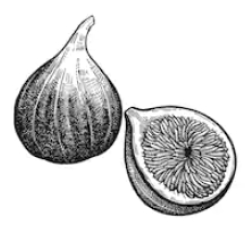
\includegraphics[width=3.3in]{figs/fig1}
	% figure caption is below the figure
	\caption{The process of scene graph generation.}
	\label{fig:1}       % Give a unique label
\end{figure}

\begin{table}
 \caption{Sample table title}
  \centering
  \begin{tabular}{lll}
    \toprule
    \multicolumn{2}{c}{Part}                   \\
    \cmidrule(r){1-2}
    Name     & Description     & Size ($\mu$m) \\
    \midrule
    Dendrite & Input terminal  & $\sim$100     \\
    Axon     & Output terminal & $\sim$10      \\
    Soma     & Cell body       & up to $10^6$  \\
    \bottomrule
  \end{tabular}
  \label{tab:table}
\end{table}


\section{Experiment}
\label{section:4}
我们通过实验分析本文提出模型Match-PRCE的性能。在VG据集上,通过与13个知名模型进行比较,来验证本文模型的有效性。同时,我们还进行了多组消融实验来进一步研究不同模块对性能的影响。
\subsection{数据集}
\subsection{评价指标}
\subsection{模型参数设置}
\subsection{实验结果}



\section{Conclusion}
\label{section:5}
结论部分总结研究的主要发现,重申其重要性,强调对理论和实践的贡献,并可能提出未来研究的方向或建议,以帮助读者理解研究的整体意义和潜在影响。

%Bibliography
\bibliographystyle{unsrt}  
\bibliography{references}  


\end{document}
